\documentclass[a4paper,10pt]{article}
\usepackage{a4wide}
\usepackage{amsmath}
\usepackage{amssymb}
%\usepackage{empheq}
\usepackage[english]{babel}
\usepackage{graphicx}
\usepackage{enumerate}
\usepackage{subcaption,array}
\usepackage{multicol}
%\usepackage{mathtools}
\usepackage{latexsym}
\usepackage{fullpage}
\usepackage{verbatim}
\usepackage{algorithm}
\usepackage{algpseudocode}
\usepackage{float}
\usepackage{bbm}
\usepackage[section]{placeins} % Prevent floats from passing beyond \FloatBarrier; keep floats within their sections
\usepackage{appendix}
\usepackage{import} %tex bestanden importeren deze moeten alleen tekst bevatten geen \begin{document} etc.
\usepackage{listings}
\usepackage{eurosym}
\usepackage[utf8]{inputenx}
\usepackage{program}
\usepackage{bookmark}

\newcommand{\desda}{\Leftrightarrow}
\newcommand{\rr}{\mathbb{R}}
\newcommand{\nn}{\mathbb{N}}
\newcommand{\zz}{\mathbb{Z}}
\newcommand{\qq}{\mathbb{Q}}
\newcommand{\rn}{\mathbb{R}^n}
\newcommand{\fdr}{f:D\rightarrow \rr}
\newcommand{\ul}{\underline}
\newcommand{\pp}{\mathbb{P}}
\newcommand{\ee}{\mathbb{E}}
\newcommand{\lnn}{\tilde{L}_n}
\newcommand{\convdis}{\overset{d}{\longrightarrow}}


\newcommand{\onaf}{\perp\!\!\!\perp}
\newcommand\red[1]{{\color{red}#1}} %kleurt text rood


\lstset{                         %settings voor code, zie ook http://en.wikibooks.org/wiki/LaTeX/Source_Code_Listings
breaklines=true,                 % sets automatic line breaking
commentstyle=\color{mygreen},    % comment style
%frame=single,                    % adds a frame around the code
keywordstyle=\color{blue},       % keyword style    \bfseries voor Bold
numberstyle=\tiny\color{black}, % the style that is used for the line-numbers
rulecolor=\color{black},         % if not set, the frame-color may be changed on line-breaks within not-black text
numbers=left,                    % where to put the line-numbers; possible values are (none, left, right)
}
\setlength\parindent{0pt}
\renewcommand\lstlistlistingname{Lijst van listings}
\usepackage{color}                  %Voor kleuren, o.a. in code
\usepackage{xcolor}                 %Voor kleuren, werkend krijgen  van box boven code
\definecolor{mygreen}{rgb}{0,0.6,0} %groene kleur voor comments in code
\usepackage{caption}
\DeclareCaptionFont{white}{\color{white}}
%\DeclareCaptionFormat{listing}{\colorbox{gray}{\parbox{\textwidth}{#1#2#3}}}
%\captionsetup[lstlisting]{format=listing,labelfont=white,textfont=white}

\usepackage{fancyhdr} %Footers en Headers
\setlength{\headheight}{15.0 pt}
\setlength{\headsep}{0.5 cm}
\pagestyle{fancy}
\fancyfoot[L]{} %naam van groep
\fancyfoot[C]{}
\fancyfoot[R]{\thepage}
\renewcommand{\footrulewidth}{0.4pt}

\fancyhead[L]{\large{\emph{Advanced simulation}}} %Naam van project
\fancyhead[C]{}
\renewcommand{\headrulewidth}{0pt} %thickness of the decorative lines on the header

\usepackage{hyperref}


\setcounter{secnumdepth}{4}% hoever de secties doornummeren
\setcounter{tocdepth}{3} %hoever de inhoudsopgave doornummert
%\setcounter{lofdepth}{2} %hoever de list of figures doornummert
%\setcounter{lotdepth}{2} % hoever de list of tables doornummert
\begin{document}
%\pagenumbering{roman}
\begin{titlepage}

\newcommand{\HRule}{\rule{\linewidth}{0.5mm}} % Defines a new command for the horizontal lines, change thickness here

\centering % Center everything on the page

%----------------------------------------------------------------------------------------
%	TITLE SECTION
%----------------------------------------------------------------------------------------
\HRule \\[0.4cm]
{ \Huge \bfseries Algorithm primitives}\\[0.4cm] % Title of your document
\HRule \\[1.5cm]

%----------------------------------------------------------------------------------------
%	HEADING SECTIONS
%----------------------------------------------------------------------------------------

%\textsc{\LARGE Technische universiteit Eindhoven}\\[1.5cm] % Name of your university/college
\textsc{\large Master Thesis}\\[1.0cm] % Minor heading such as course title vakcode
%----------------------------------------------------------------------------------------
%	LOGO SECTION
%----------------------------------------------------------------------------------------

%\fbox{\includegraphics[width=0.8\textwidth]{bus.png}}\\[1cm] % Include a department/university logo - this will require the graphicx package

%----------------------------------------------------------------------------------------
%	AUTHOR SECTION
%----------------------------------------------------------------------------------------
\vfill % Fill the rest of the page with whitespace
% Alles onder elkaar

L.D. Stooker, 0819041 \\ [1cm]


%----------------------------------------------------------------------------------------
%	DATE SECTION
%----------------------------------------------------------------------------------------

{\large \today}\\[3cm] % Date, change the \today to a set date if you want to be precise



%----------------------------------------------------------------------------------------



\end{titlepage}

\begin{abstract}
To improve existing automated picking of a machine learning algorithm

\end{abstract}

\newpage
\tableofcontents
\newpage


\section{Introduction} \label{Chapter1}
This report is the result of my graduation project which completes my Business Information Systems study at Eindhoven University of Technology.
The project was performed internally at the University in the Data mining department.
In this project we investigated annotations of primitives, more specifically primitives in the scikit-learn library.
In the section \ref{Intr-Prob} we will briefly explain more about primitives and the annotations.
To elaborate on this we will outline the research questions and thesis structure
 

\subsection{problem description}\label{Intr-Prob}
Machine learning is a growing field that can help process the increase of available data\cite{Big-data}\cite{ML-trends}. 
Python is a langauge which holds premade machine learning algorithms in libaries like scikit-learn\cite{scikit-learn}.
In recent years python is also increasing in so called market share for machine learning\cite{python-pop}.
To help machine learners using the scikit-learn library made a model to indicate what algorithm to use for what problem. 
In this model (\ref{fig:FlowChartML}) you can see that depending on size of the data and early results different algorithms are recommened. 

\begin{figure}[h] %use t for top of page instead of h for here
	\centering
	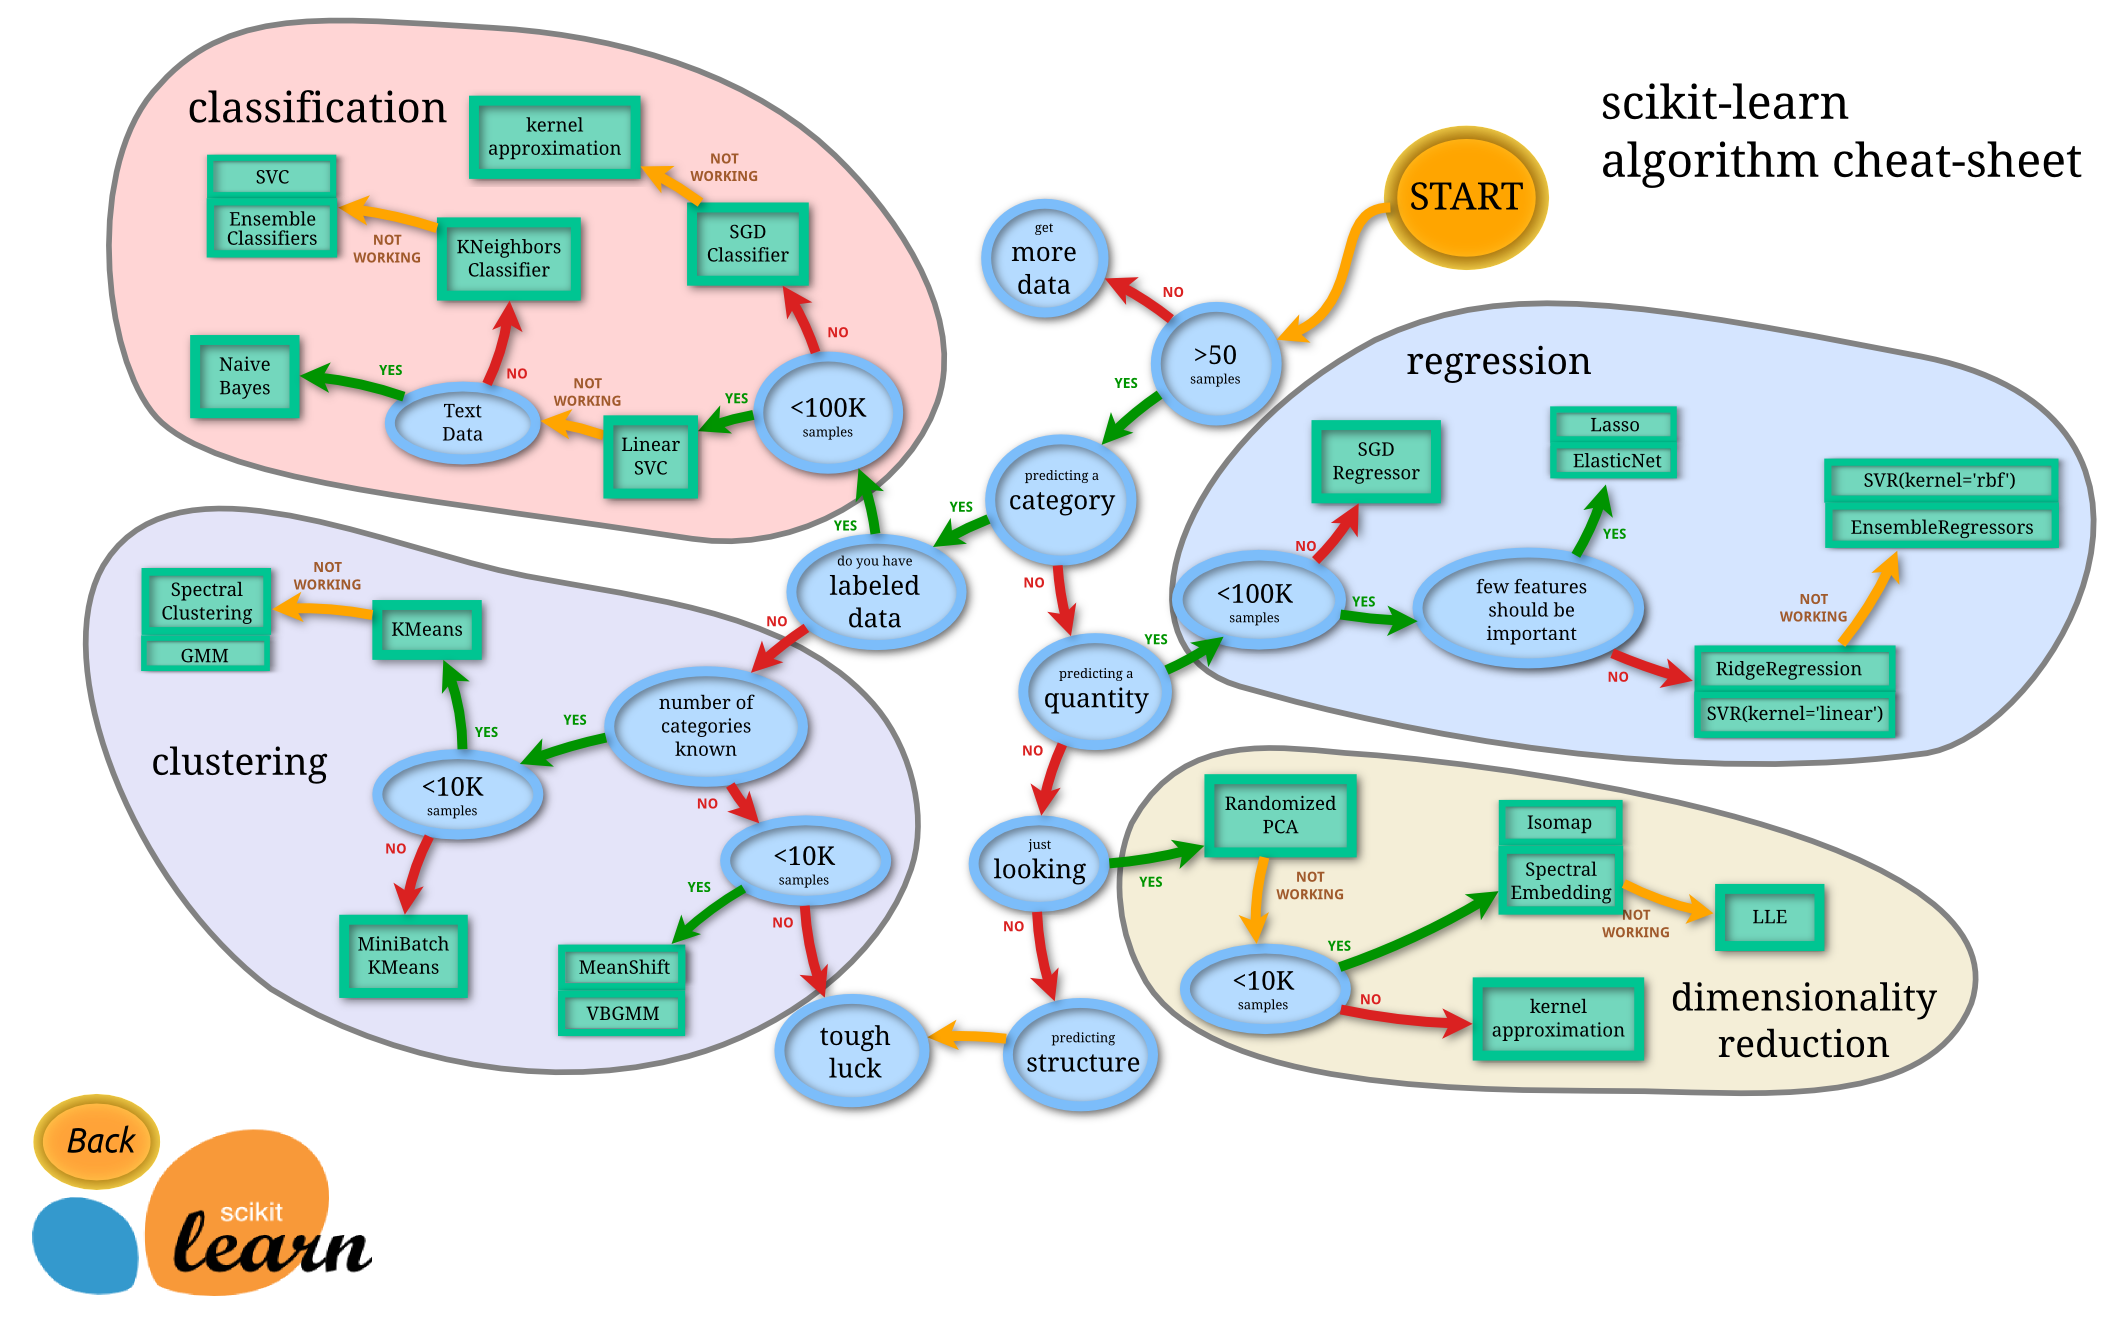
\includegraphics[
	width=0.65\textwidth
	]{images/FlowChartML.png}
	\caption{FlowChartML}
	\label{fig:FlowChartML}
\end{figure}
%explain the need for automation and then the boost of information, I try to give.

\subsection{research question}
% the proposed annotations
We base our research question on the work of Joaquin to give properties to algorithms. More specifially we look more closely to the resilience properties. 

\subsection{thesis structure}

\subsection{Outline}

\newpage


\section{Preliminaries} \label{Chapter2}
Before we discuss in detail the solutions for the steps of our approach, this chapter provides
some background knowledge and definitions which are required for a good understanding of
the remainder of this thesis.
\subsection{Sklearn/scikit-learn library}
%subsubsections for algorithms?
% Include the chart of sklearn which algorithm to pick

\subsection{Terminology}

\newpage
\section{Experimental setup} \label{Chapter3}
\subsection{Motivation} \label{motivation}


\newpage
\subsection{Description} \label{description}


\subsubsection{Main method}


\subsubsection{Strategy 1}


\subsubsection{Strategy 2}


\subsubsection{Strategy 3}


\subsubsection{Strategy 4}


\subsubsection{Strategy 5}




\subsubsection{Strategy 6}



\subsection{Realist model} \label{realistic}


\newpage 

\section{Experimental Results} \label{Chapter4}

\subsubsection{Main method}


\subsubsection{Strategy 1}


\subsubsection{Strategy 2} 



\subsubsection{Strategy 3}


\subsubsection{Strategy 4}



\subsubsection{Strategy 5}


\subsubsection{Strategy 6}

\section{Discussion} \label{Chapter5}

\newpage
\section{Conclusion} \label{Chapter6}

\section{References}
\begingroup
\begin{thebibliography}{9}
\bibitem{Data-science} The Popularity of Data Science Software, Robert A. Muenchen, r4stats.com, (2017)
\bibitem{python-pop} Most Popular Programming Languages For Machine Learning And Data Science,Adarsh Verma, fossbytes.com, (2016)
\bibitem{ML-trends} 
Machine learning: Trends, perspectives, and prospects, M. I. Jordan, T. M. Mitchell, Science Volume 349 issue 6245 pages 255-260, (2015)
\bibitem{Big-data} Storage predictions: Will the explosion of data in 2017 be repeated in 2018?, Nick Ismail, www.information-age.com/, (2017)
     
\end{thebibliography}
\endgroup

\end{document}